%intro
One of the purposes of doing incremental reconstruction is to be able to see the volume as it is constructed. This allows for immediate feedback during scanning. There are many ways to visualize a volume, and the system described in this thesis offers orthogonal multiplanar reformatting (MPR) slices or volume ray casting. In addition, as the volume is accessible on both device and host memory, it can be used as input for third-party visualization packages. In this section, the visualization techniques used are described.

\subsection{Orthogonal MPR slices}
% pictchaz
% volume on CPU, slices extracted (no interpolation because of orthogonal along axis)
% how used OpenGL
% explain user interface (mouse rotate and index incr/decr)

\begin{figure}[h]
\centering
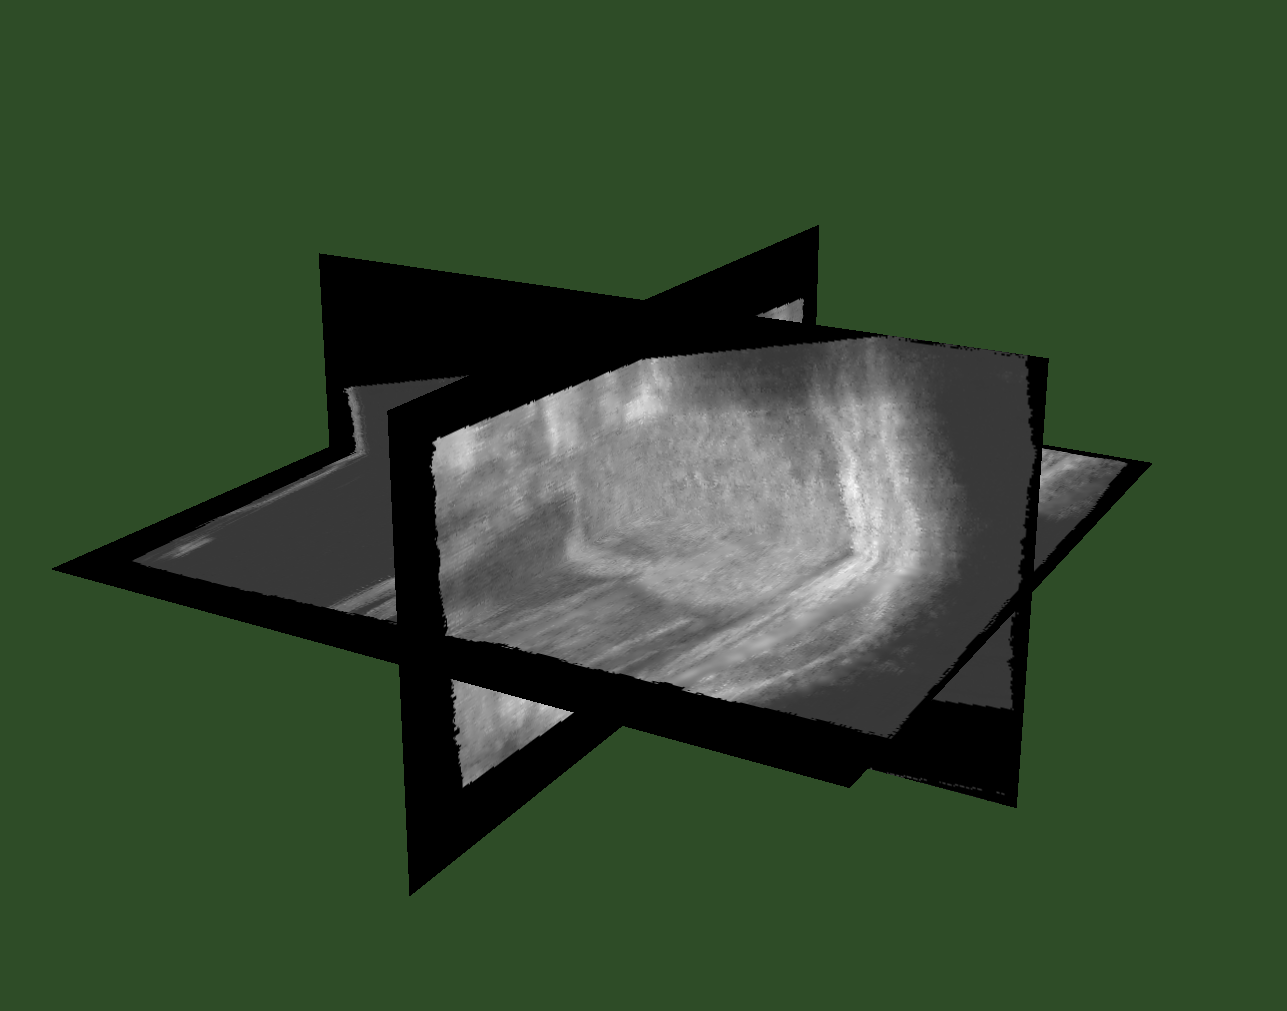
\includegraphics[width=0.49\textwidth]{graphics/orthogonal_screen0.png}
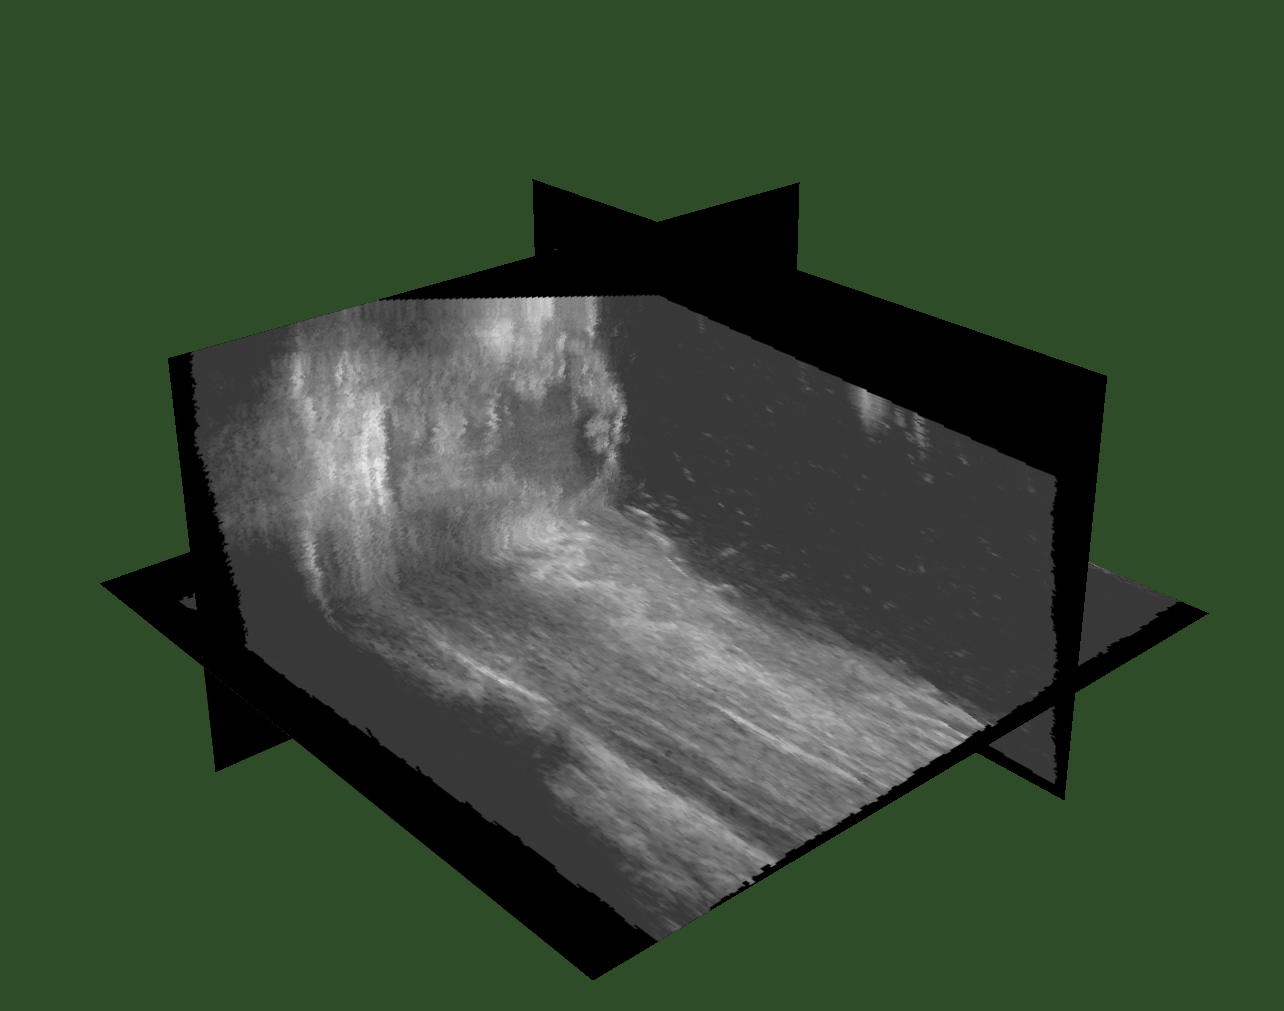
\includegraphics[width=0.49\textwidth]{graphics/orthogonal_screen1.png}
\caption[Screenshots of orthogonal MPR slices]{Screenshots of orthogonal MPR slices generated by our implementation}
\label{fig:orthogonal_screens}
\end{figure}

Figure \ref{fig:orthogonal_screens} shows some screenshots of the orthogonal MPR slices, and larger figures can be found in Appendix \ref{chapter:large_figures}. The slices are along each of the three volume axis, and the voxel values in each slice are rendered on the slice plane. This is performed by extracting voxel values on indices $(x,y,i)$, $(x,i,z)$ and $(i,y,z)$ for the z, y and x axis, respectively. The parameter $i$ determines where on each axis the slices are located, while $x$, $y$ and $z$ are all the possible voxel indices in the volume. The slices are extracted from the host memory volume and used as textures for three orthogonal polygons rendered with OpenGL. It should be noted that extracting the voxels and using them as textures takes a negligible amount of time. Using the mouse, the user can rotate the volume to view the slices at different angles, and pressing keyboard keys will increase or decrease the $i$ parameter. In this way, all parts of the volume can be visualized.

\subsection{Volume Ray Casting}
% pictchaz
% volume ray casted while on GPU
% one thread per ray
% build ray dirs kernel
% cast rays kernel
% do box-ray intersection to skip to volume before stepping
% set strength to max_voxel
% for each step:
	% if strength below cutoff -> end stepping
	% calculate transparency: min(1-voxel/max_voxel + adjustment, 1)
	% (if voxel below (other) cutoff -> set transparent to 1 (due to grey US background))
	% accumulate strength*(1-transparency)
	% update strength by multiplying with transparency
% set pixel to ray accumulation

\begin{figure}[h]
\centering
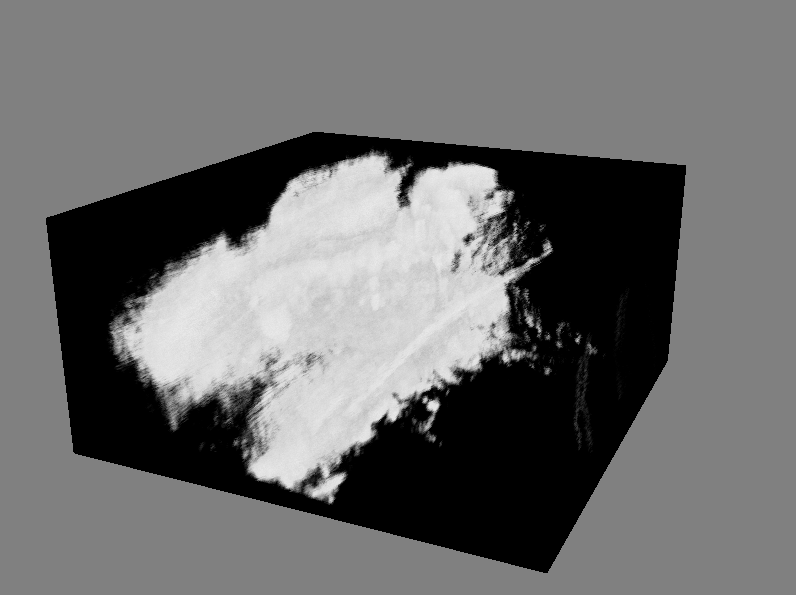
\includegraphics[width=0.49\textwidth]{graphics/raycast_screen0.png}
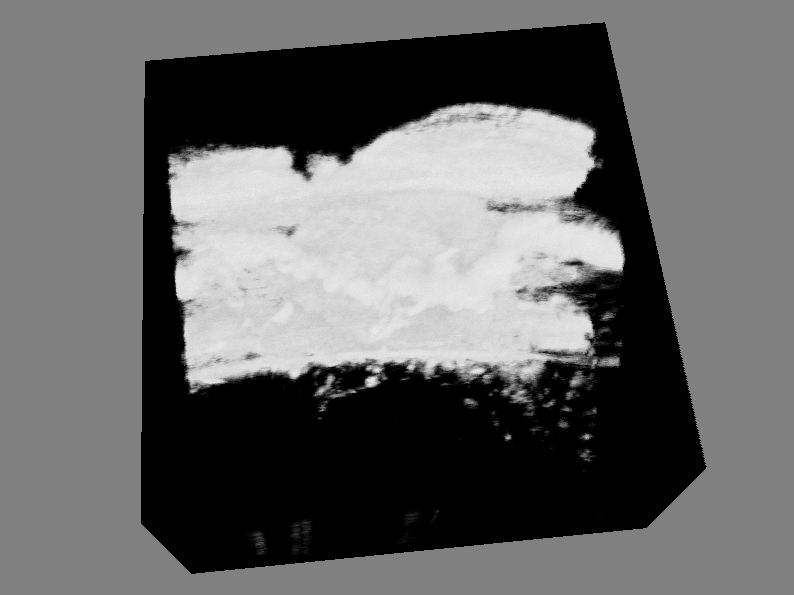
\includegraphics[width=0.49\textwidth]{graphics/raycast_screen1.png}
\caption[Screenshots of volume ray casting]{Screenshots of volume ray casting generated by our implementation}
\label{fig:raycast_screens}
\end{figure}

Figure \ref{fig:raycast_screens} shows some screenshots of the ray casted volume, and larger figures can be found in Appendix \ref{chapter:large_figures}. Ray casting is a computationally demanding task, but the GPU's processing power is utilized while the volume data is still on the device memory. The task is parallelized with one thread per ray, and consists of two steps: first construct the rays, then cast them into the volume.

Code listings of the implemented OpenCL kernels can be found in Appendix \ref{section:ray_casting_kernel}. The resulting rendered image consists of $w_s \times h_s$ pixels, with one ray (and thread) per pixel. The camera is defined by a camera location in space, a \emph{lookat} location that the camera is looking at, a vector defining "up" in the rendered image, and a vector defining "flat" (the horizontal direction) in the rendered image. Each ray's origin is the given camera location, but their direction needs to be calculated from their pixel position and a desired field-of-view. %This is done with Equation \ref{eq:ray_dir}.

%\begin{equation}
%	\label{eq:ray_dir}
%	r = \left| |camera_{lookat}-camera_{pos}| + FOV_{hor} camera_{right} \frac{x_{ray} - \frac{w_s}{2}}{\frac{w_s}{2}} + FOV_{vert} camera_{up} \frac{y_{ray} - \frac{h_s}{2}}{\frac{h_s}{2}} \right|
%\end{equation}

When the ray directions have been found, they can be cast into the volume. Instead of stepping from the ray origin, we save computations by first calculating the intersection between the box-shaped volume and each ray. This saves sampling for steps that are outside the volume.

There are many ways to accumulate voxel intensities while stepping along a ray. The method used in this work models the voxels as transparent cubes with a transparency level between 0.0 (fully oblique) and 1.0 (invisible). The entire procedure is as follows:

\begin{enumerate}
	\item $strength = 255$
	\item for each step along ray:
	\begin{enumerate}
		\item if $strength <$ cutoff, then break stepping
		\item $transparency = 1-\frac{intensity_{voxel}}{255}$
		\item accumulate $strength \cdot (1-transparency)$ into ray's pixel intensity
		\item $strength \leftarrow strength \cdot transparency$
	\end{enumerate}
\end{enumerate}

Each ray starts with a \emph{strength} parameter representing how much light has been absorbed. The initial value is the maximum value of a pixel (255), and it is reduced for each voxel encountered. For each voxel sampled, its intensity is weighted by the current strength and accumulated into the final pixel intensity. To save computations, the stepping is ended if the strength is below a given cutoff where the voxels simply do not contribute noticeable intensities.